\documentclass[12pt,compress]{beamer}
\usepackage{ifthen}

\title{A Validation Suite/Simple Alignment Algorithm for Muon Chambers}
\author{Jim Pivarski}
\institute{Texas A\&M University}
\date{27 October, 2006}

\setbeamertemplate{navigation symbols}{}
\setbeamertemplate{headline}{\includegraphics[height=1 cm]{../cmslogo} \hspace{0.1 cm} \includegraphics[height=1 cm]{../tamulogo} \hfill
\begin{minipage}{9 cm}
\vspace{-0.75 cm} \small
\begin{center}
\ifthenelse{\equal{\insertpagenumber}{1}}{}{\insertsection}
\end{center}
\end{minipage} \hfill
\begin{minipage}{1 cm}
\vspace{-0.75 cm} \small
\begin{center}
\ifthenelse{\equal{\insertpagenumber}{1}}{}{\insertpagenumber/\pageref{numpages}}
\end{center}
\end{minipage}}

\xdefinecolor{verylightgray}{rgb}{0.95,0.95,0.95}
\beamertemplateshadingbackground{verylightgray}{white}

\begin{document}
\frame{\titlepage}
\section*{Validation and Simple Alignment --- Jim Pivarski}

\begin{frame}
\frametitle{Context}

Three sophisticated alignment algorithms have been developed over the past 3 years:

\begin{description}
\item[HIP] iterative $\chi^2$ minimization of residuals
\item[Millepede] matrix inversion, at least in spirit
\item[Kalman] coupled track-fitting and alignment
\end{description}

\vfill Possible disadvantage: they are all global fits, it may be hard
to diagnose problems with individual chambers

\vfill Misalignment distribution may be very non-Gaussian due to
static friction: some chambers stick while others slip\ldots
\end{frame}

\begin{frame}
\frametitle{Si-Vertex Alignment at the CLEO Experiment}
\begin{itemize}
\item Global fit did not reliably reduce $\chi^2$
\item Plotted residuals for and corrected each wafer individually
\end{itemize}
\begin{center}
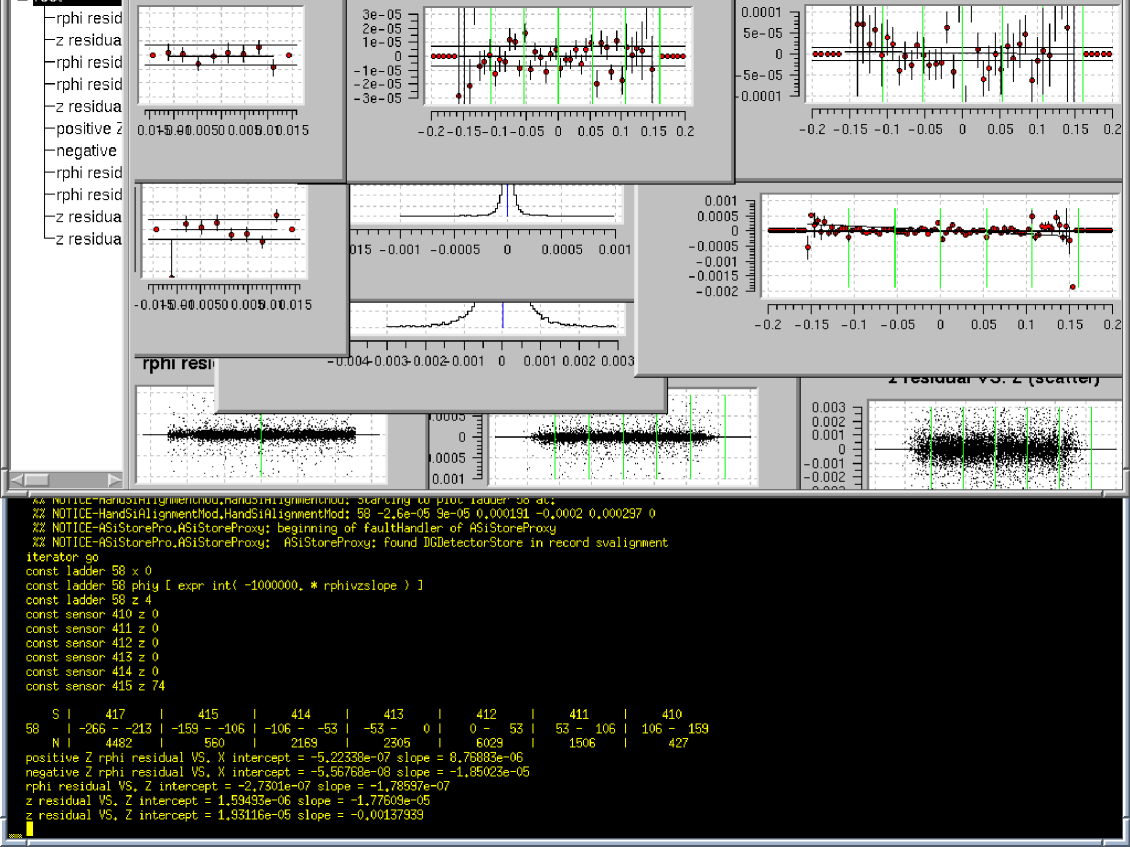
\includegraphics[width=0.75\linewidth]{hand_alignment2}
\end{center}
\end{frame}

\begin{frame}
\frametitle{Five Degrees of Freedom from a 2D Sensor}

$r_x$ $=$ track$-$hit residual in local coordinate $x$

\vspace{-1 cm}
\begin{center}
\begin{tabular}{p{0.31\linewidth} p{0.31\linewidth} p{0.31\linewidth}}
  \begin{minipage}{\linewidth}
    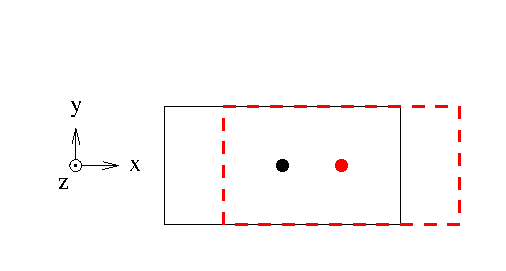
\includegraphics[width=\linewidth]{dof_x}
  \end{minipage} &
  \begin{minipage}{\linewidth}
    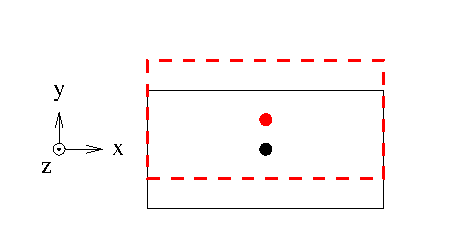
\includegraphics[width=\linewidth]{dof_y}
  \end{minipage} &
  \begin{minipage}{\linewidth}
    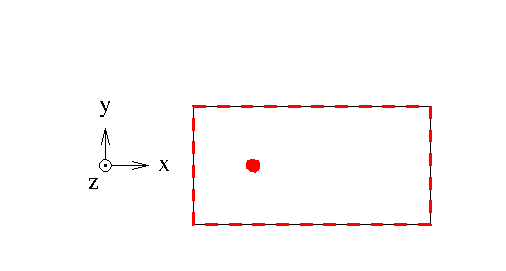
\includegraphics[width=\linewidth]{dof_z}
  \end{minipage} \\
  \begin{minipage}{\linewidth}
    \begin{center}
      $x$: offset in $r_x$
    \end{center}
  \end{minipage} &
  \begin{minipage}{\linewidth}
    \begin{center}
      $y$: offset in $r_y$
    \end{center}
  \end{minipage} &
  \begin{minipage}{\linewidth}
    \begin{center}
      $z$: inaccessible
    \end{center}
  \end{minipage} \\
  & & \\
  \begin{minipage}{\linewidth}
    \tiny
    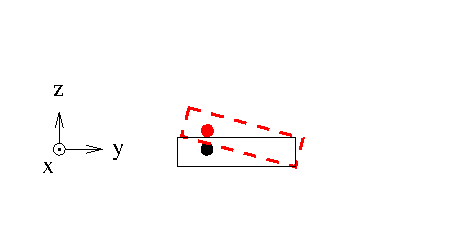
\includegraphics[width=\linewidth]{dof_phix} \\ \mbox{ }
  \end{minipage} &
  \begin{minipage}{\linewidth}
    \tiny
    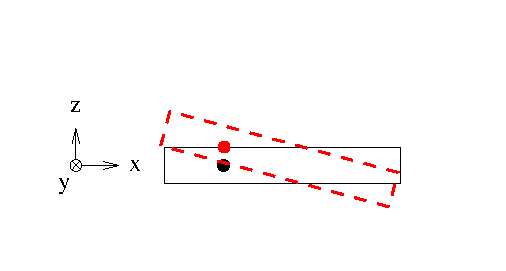
\includegraphics[width=\linewidth]{dof_phiy} \\ \mbox{ }
  \end{minipage} &
  \begin{minipage}{\linewidth}
    \tiny
    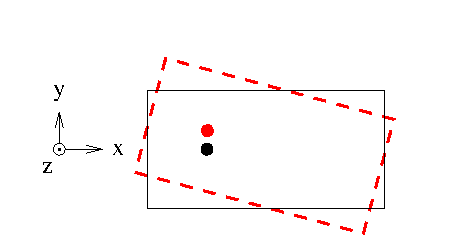
\includegraphics[width=\linewidth]{dof_phiz} \\ \mbox{ }
  \end{minipage} \\
  \begin{minipage}{\linewidth}
    \begin{center}
      $\phi_x$: $r_y$ linear in $y$ \\ \mbox{ }
    \end{center}
  \end{minipage} &
  \begin{minipage}{\linewidth}
    \begin{center}
      $\phi_y$: $r_x$ linear in $x$ \\ \mbox{ }
    \end{center}
  \end{minipage} &
  \begin{minipage}{\linewidth}
    \begin{center}
      $\phi_z$: $r_x$ linear in $y$ and $r_y$ linear in $x$
    \end{center}
  \end{minipage} \\
  \begin{minipage}{\linewidth}
    \scriptsize
    \begin{center}
      (slope $=$ $1 - \cos\phi_x$)
    \end{center}
  \end{minipage} &
  \begin{minipage}{\linewidth}
    \scriptsize
    \begin{center}
      (slope $=$ $1 - \cos\phi_y$)
    \end{center}
  \end{minipage} &
  \begin{minipage}{\linewidth}
    \scriptsize
    \begin{center}
      (slope $=$ $\sin\phi_z$)
    \end{center}
  \end{minipage}
\end{tabular}
\end{center}

\end{frame}

\begin{frame}
\frametitle{Example from CLEO}

\begin{columns}
\column{0.35\linewidth}
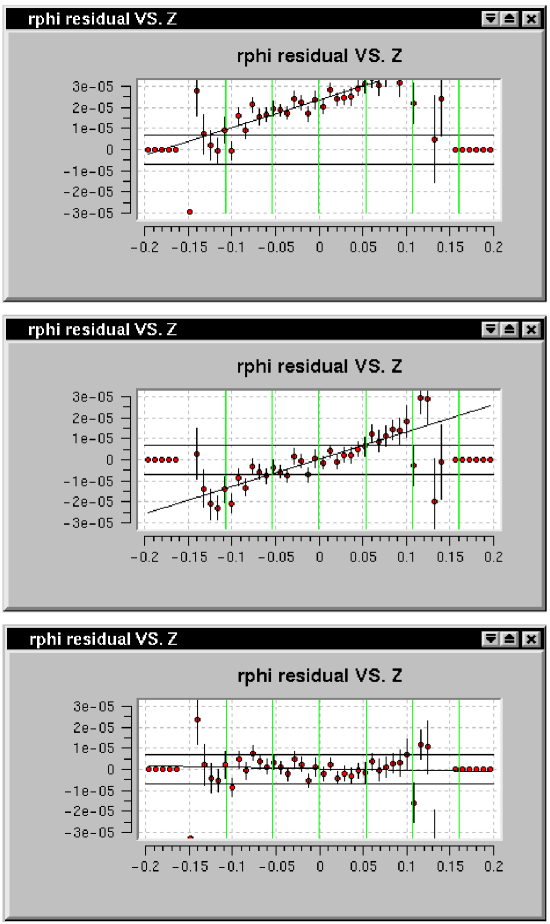
\includegraphics[width=\linewidth]{hand_alignment3}
\column{0.7\linewidth}

Take this plot to be $r_x$ versus $y$ \\
(ignore the different axis label convention)

\begin{enumerate}
  \item Linear fit to profile plot
  \item Shift $x$ position to correct offset
  \item Rotate $\phi_z$ to correct slope
  \item Apply similar corrections to the degrees of freedom not shown
  \item Iterate to resolve correlations
\end{enumerate}

Not an efficient or an elegant alignment procedure, but you can see what's happening
\end{columns}
\end{frame}

\begin{frame}
\frametitle{Muons: Simpler with Segments?}

\begin{columns}
\column{0.25\linewidth}
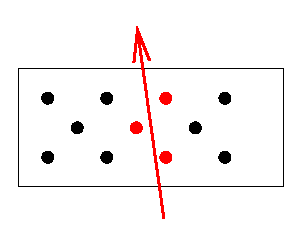
\includegraphics[width=\linewidth]{simpler_with_segments}
\column{0.7\linewidth}
Muon code reconstructs local 4D segments (2D position $+$ 2D direction)
\end{columns}

\vfill
Angular track$-$segment difference in $x$-$z$ plane is $\phi_y$

Angular track$-$segment difference in $y$-$z$ plane is $\phi_x$

\vspace{0.2 cm}
Replace weak $\mathcal{O}(\phi^2)$ dependencies!

\vfill
{\bf But,}
\begin{itemize}
  \item need to propagate to segment's local coordinate system (center
  of chamber, not the layer plane)
  \item may require substantial re-working of CommonAlignment
  \item other subtleties I don't understand yet\ldots
\end{itemize}
\end{frame}

\begin{frame}
\frametitle{Another Useful Diagnostic}
\begin{columns}
\column{0.4\linewidth}
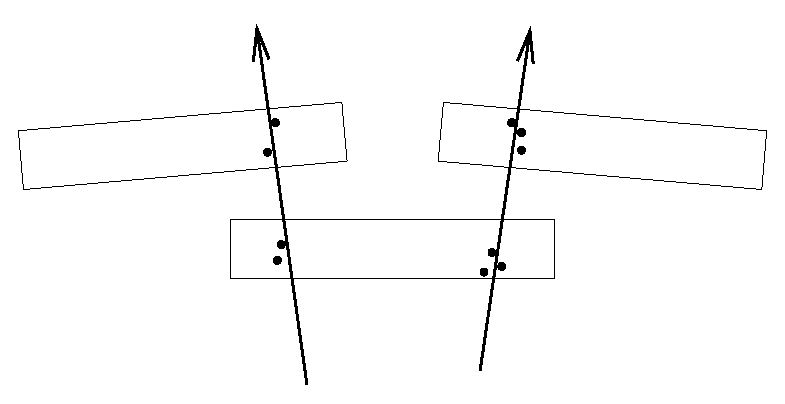
\includegraphics[width=\linewidth]{overlap_plots}
\column{0.55\linewidth}
Local consistency of the overlap regions (track has hits in two
chambers in the same layer)
\end{columns}

\vfill Easy way to implement: $\mbox{residual}_{\mbox{\scriptsize chamber 1}} - \mbox{residual}_{\mbox{\scriptsize chamber 2}}$

\vfill (track cancels, effectively a ``ruler'' curved in the $\vec{B}$ field)

\vfill
{\bf But,}
\begin{itemize}
  \item hard to interpret as a correction: diagnostic only
  \item low statistics
\end{itemize}



\end{frame}

\begin{frame}
\frametitle{Possible Future Timeline}

\renewcommand{\arraystretch}{3.3}
\begin{tabular}{p\linewidth}
  \begin{minipage}{0.55\linewidth}
    \begin{enumerate}
    \item Test Residuals Algorithm in MuonAlignmentAnalyzer
    \end{enumerate}
  \end{minipage}
  \begin{minipage}{0.43\linewidth}
    \begin{enumerate}
    \item Add muon chambers to CommonAlignment
    \end{enumerate}
  \end{minipage} \\
  \begin{minipage}{\linewidth}
    \begin{enumerate}
      \addtocounter{enumi}{1}
    \item Incorporate Residuals Algorithm into CommonAlignment
    \end{enumerate}
  \end{minipage} \\
  \begin{minipage}{0.55\linewidth}
    \begin{enumerate}
      \addtocounter{enumi}{2}
    \item Apply Residuals Algorithm to early data, possibly only the largest outliers
    \end{enumerate}
  \end{minipage}
  \begin{minipage}{0.43\linewidth}
    \begin{enumerate}
      \addtocounter{enumi}{2}
    \item Use it to debug global fits, if necessary \\ \mbox{ }
    \end{enumerate}
  \end{minipage} \\
  \begin{minipage}{\linewidth}
    \begin{enumerate}
      \addtocounter{enumi}{3}
    \item Use residuals plots to monitor global fits, which do the real alignment
    \end{enumerate}
  \end{minipage}
\end{tabular}
\label{numpages}
\end{frame}

\end{document}
